\section{ТЕОРЕТИЧЕСКИЕ ОСНОВЫ СВЕРТОЧНЫХ СЕТЕЙ}

\subsection{Общая теория глубокого обучения}

Прежде чем говорить о сверточных нейронных сетях, стоит рассмотреть ключевые понятия в теории глубокого обучения.
Самой базовой моделью глубокого обучения называется так называемый \textbf{многослойный перцептрон}, или \textbf{MLP}.

Основная идея данной модели заключается в построении отдельных слоев линейных моделей, называемых \textbf{перцептронами}, связанных со всеми моделями следующего слоя некой нелинейной функцией,
называемой \textbf{функцией активации}. На рисунке \ref{fig:mlp} изображена примерная схема MLP, где каждая стрелка означает вход с применением функции активации.

\begin{figure}[h]
    \centering
    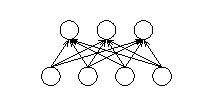
\includegraphics[width=0.8\textwidth]{images/mlp.pdf}
    \caption{Схематичное изображение MLP}
    \label{fig:mlp}
\end{figure}

Используют различные функции активации.
В конце XX века чаще использовали сигмоидные функции $\text{tahn}(x) = \frac{2}{1 + e^{-2x}} - 1$ и $\sigma(x) = \frac{1}{1 + e^{-1x}}$.
Изображение этих функций представлено на рисунке \ref{fig:sigmoids}.

\newpage
\begin{figure}[h]
    \centering
    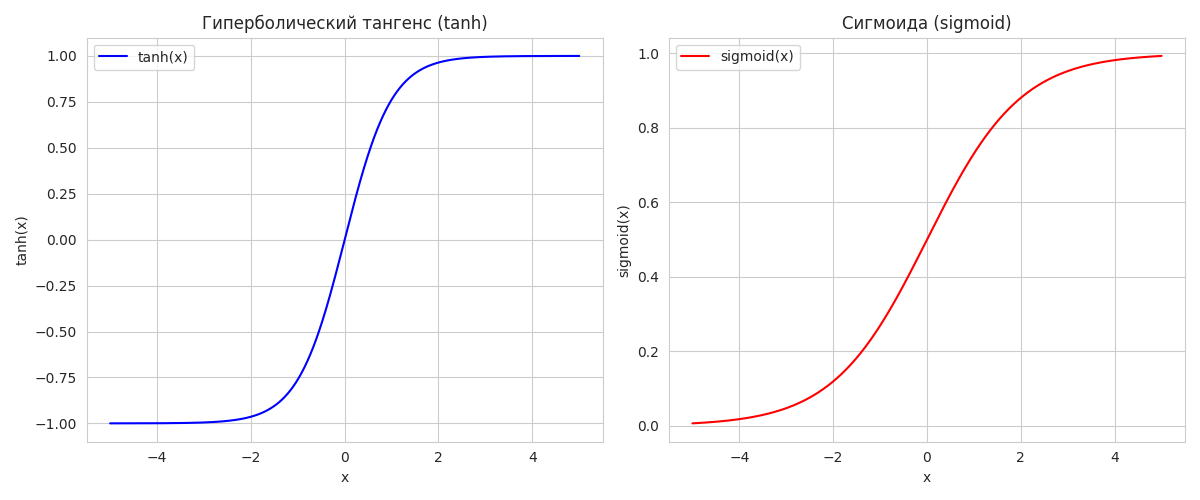
\includegraphics[width=1.0\textwidth]{images/sigmoids.png}
    \caption{Сигмоидные функции активации}
    \label{fig:sigmoids}
\end{figure}

Современные нейросетевые решения используют функцию активации \\
$\text{ReLU}(x) = \frac{x + |x|}{2} = \max(0, x)$ (rectified linear unit).
Ее изображение представлено на рисунке \ref{fig:relu}.

\begin{figure}[h]
    \centering
    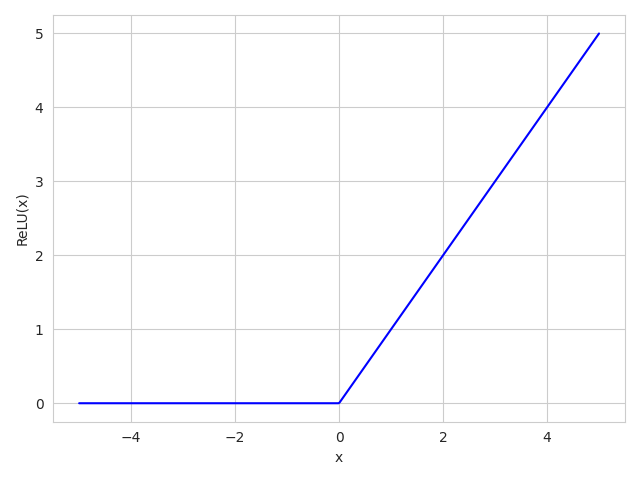
\includegraphics[width=0.8\textwidth]{images/relu.png}
    \caption{Функция активации ReLU}
    \label{fig:relu}
\end{figure}

Популярность функции ReLU связана с проблемой затухающих градиентов \cite{dlbook}.
Вне окрестности нуля сигмоидные функции имеют очень малые значения производной, что негативно сказывается на обучении модели.

Теперь рассмотрим, каким образом будет выглядеть выходная функция, преобразующая исходный вектор $x$ в вектор $z$ последнего слоя.
Под слоем теперь будем подразумевать произвольную дифференцируемую (за исключением счетного числа точек) функцию многих переменных $x$ и $w$.
Если модель имеет $l$ слоев $f_l, \ldots, f_1$ с параметрами $w_l, \ldots, w_1$ на каждом слое, то выходную функцию можно представить в виде:
\begin{equation}
    z = f_l(w_l, f_{l-1}(\ldots f_1(w_1, x))\ldots)) = \hat{f}(x, \omega_1, \ldots, \omega_l)
\end{equation}

Таким образом, нейросеть представляет собой композицию параметрических функций \cite{VorontsovML}.
Поставленную задачу можно в общем случае описать как аппроксимацию некой функции $z = f(x)$ с помощью композиции параметрических функций.
Для идентификации неизвестных параметров $w_i, i = 1, \ldots, l$ необходим набор пар $(x_i, y_i)$, где $y = f(x)$ и $i = 1, \ldots, N$, $N$ -- размер обучаемого набора.

Задачу подбора параметров модели решают с помощью введения скалярной функции многих переменных, называемой \textbf{функцией потерь}, которая зависит от точных значений выходных переменных $y = f(x)$ и выходных переменных модели $\hat{y} = \hat{f}(x, \omega_1, \ldots, \omega_l)$.
Данная функция характеризует, насколько точно модель предсказывает истинные значения $y$.
Решая задачу минимизации (максимизации) данной функции, получаем некоторую оценку истинных параметров модели.

В задаче классификации используют функцию потерь, называемую \textbf{перекрестной энтропией}, или \textbf{crossentropy loss} \cite{VorontsovML}.
Как правило, выходной слой классификационной модели интерпретируется как вектор вероятностей классификации каждого класса.
Математически перекрестная энтропия описывается так:
\begin{equation}
    H = \frac{1}{N} \sum_{i = 1}^{N} \log(P(y_i = \hat{y}_i\ |\ x_i, w)),
\end{equation}
где $P(y = \hat{y}\ |\ x, w)$ -- вероятность значения $y_i$, предсказанная моделью.

Для минимизации функции потерь на практике используют алгоритм градиентного спуска или его модификации.
Для оптимального вычисления градиентов в нейрнонных сетях был разработан специальный алгоритм \textbf{backpropagation} \cite{backprop}.

\subsection{Сверточные нейронные сети}

Определим операцию дискретной свертки двух последовательностей $x = \{x_i\},\ y = \{y_i\}$:
\begin{equation}
    (x * y)(t) = \sum_{i} x_i \cdot y_{t - i}
\end{equation}

Аналогично можно определить двумерную свертку для двумерных последовательностей $X = \{X_{i,j}\},\ Y = \{Y_{i,j}\}$:
\begin{equation}
    (X * Y)(t, s) = \sum_{i, j} X_{i,j} \cdot Y_{t - i, s - j}
\end{equation}

Если же двумерные векторы конечны, то есть их можно представить в виде матриц, операцию свертки интерпретируют как наложение окна $Y$ с симметрией относительно побочной диагонали и сдвигом на $(t, s)$ на матрицу $X$, с последующим суммированием (рисунок \ref{fig:conv_window}).
Таким образом, свертка в точке $(t, s)$ максимальна, когда матрица $X$ равна повернутой матрице $Y$ со сдвигом на $(t, s)$.

\begin{figure}[h]
    \centering
    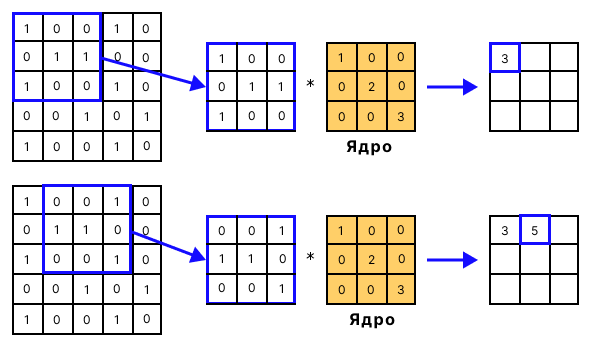
\includegraphics[width=0.7\textwidth]{images/conv_window.png}
    \caption{Визуализация операции свертки с "перевернутым" ядром}
    \label{fig:conv_window}
\end{figure}

В связи с неудобством рассмотрения повернутой матрицы $Y$ под сверткой часто подразумевают несколько иную операцию, называемой \textbf{взаимной корреляцией} \cite{dlbook}:
\begin{equation}
    (X \otimes Y)(t, s) = \sum_{i, j} X_{i, j} \cdot Y_{i + t, j + s}
\end{equation}
Такая операция теряет свойство симметричности, однако удобнее в своей интерпретируемости.
В дальнейшем под двумерной сверткой будет подразумеваться именно взаимная корреляция.

Одним из способов анализировать изображения, который использовали до появления современных алгоритмов машинного обучения, является метод матричных фильтров.
Рассмотрим изображение в черно-белом формате разрешения $n \times m$:
\[
    X = \begin{pmatrix}
        X_{11} & \ldots & X_{1m} \\
        \vdots & \ldots & \vdots \\
        X_{n1} & \ldots & X_{nm}
    \end{pmatrix}
\]
Фильтром размера $k \times l$, где $k < n,\ l < m$ назовем матрицу:
\[
    K = \begin{pmatrix}
        K_{11} & \ldots & X_{1l} \\
        \vdots & \ldots & \vdots \\
        K_{k1} & \ldots & K_{kl}
    \end{pmatrix}
\]
Метод фильтров подразумевает вычисление свертки матрицы и фильтра.
Подбирая подходящий фильтр и смотря на величину свертки, можно производить анализ изображения.
Например, если фильтр характеризует "границу" некоторого объекта, по значению свертки можно выделить эту границу.

\textbf{Сверточным слоем} в нейронной сети будем называть слой, преобразующий входную переменную $x$ в свертку этой переменной с \textbf{ядром} слоя $k$:
\[
    z = k \otimes x
\]
Использование сверточных слоев в случае, когда входной переменной является матрица (например, изображение), обосновывается методом фильтров, который успешно применяли в прошлом.

Сверточный слой отличается от полносвязного тем, что нейроны следующего слоя связаны с предыдущими локально.
Локальность в случае одномерных слоев представлена на рисунке \ref{fig:conv}.

\begin{figure}[ht]
    \centering
    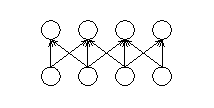
\includegraphics[width=0.8\textwidth]{images/conv.pdf}
    \caption{Локальность сверточных слоев}
    \label{fig:conv}
\end{figure}

На практике сверточные слои дополнительно модифицируют.
Помимо размера ядра, есть параметры "padding" и "stride".
Параметр padding дополняет входную матрицу нулями по краям, чтобы выходной вектор был другого размера.
Параметр stride влияет на то, сколько сверток "пропускается".
Пример того, как выглядит сеть при $\text{stride} = 2$, представлен на рисунке \ref{fig:stride}.

\begin{figure}[h]
    \centering
    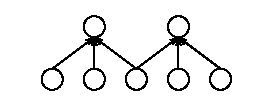
\includegraphics[width=0.8\textwidth]{images/stride.pdf}
    \caption{Вид сверточного слоя при $\text{stride}=2$}
    \label{fig:stride}
\end{figure}

Помимо сверточных слоев при построении CNN важно добавлять "pooling" слои.
В отличие от сверточных ядер, ядро pooling слоя является непараметрической функцией от "окна".
На практике используют "max pooling" (максимум) и "average pooling" (среднее) слои.
Параметры "padding" и "stride" для pooling слоев работают также, как и для сверточных.

При построении моделей на каждом слое подбирается несколько фильтров, у каждого из которых есть своя матрица на выходе.
Выходную матрицу одной свертки называют \textbf{каналом}.
В общем случае на входе сверточного слоя находится тензор 3-го порядка $X_{ijk}$, где $i$ -- номер канала, $j$ и $k$ -- пространственные координаты.
Ядро каждого канала также становится трехмерным.
Общая формула свертки:
\begin{equation}
    \text{conv}(X, K)_{i'j'k'} = \sum_{i, j, k} X_{i,j+j',k+k'} K_{i'ijk},
\end{equation}
где в ядре $K_{i'ijk}$ индекс $j'$ определяет номер выходного канала, $j$ -- номер входного канала.

\subsection{Нормализация слоев}
Между сверточными, pooling и полносвязными слоями можно ставить вспомогательные слои, выполняющие различные функции.
При решении поставленной задачи использовались 3 подобных слоя, а именно: "batch" нормализация, "local response" нормализация, и "dropout" нормализация.

\textbf{Batch} нормализация используется между слоем и его функцией активации. Его используют в случае, когда на вход модели подается параллельно сразу M входных изображений, называемых батчем размера M.
Сначала происходит нормализация "по батчу", то есть вычисление среднего и дисперсии:
\begin{equation}
    \begin{gathered}
        \mu_{jk} = \frac{1}{M} \sum_{i = 1}^{M} X_{ijk} \\
        \sigma_{jk} = \frac{1}{M} \sum_{i = 1}^{M} (X_{ijk} - \mu_{jk})^2
    \end{gathered}
\end{equation}
Затем входной вектор нормализуется:
\begin{equation}
    \hat{X}_{ijk} = \frac{X_{ijk} - \mu_{jk}}{\sqrt{\sigma_{jk}^2 + \varepsilon}}
\end{equation}
Последним этапом batch нормализации является масштабирование:
\begin{equation}
    Y_{ijk} = \gamma_{jk} \hat{X}_{ijk} + \beta_{jk},
\end{equation}
где $\gamma_{jk}$ и $\beta_{jk}$ являются обучаемыми параметрами.
Засчет масштабирования в конце модель может "отменить" проделанную нормализацию, если это необходимо \cite{batch}.

\textbf{Local response} нормализация усредняет выход нейронного слоя по каналам \cite{alexnet}:
\begin{equation}
    Y_{c} = X_{c} \left( k + \frac{\alpha}{n}\sum_{c' = \max(0, c - \frac{n}{2})}^{\min(N - 1, c + \frac{n}{2})} X_{c'} \right)^{-\beta},
\end{equation}
где $X_c$ -- канал, $k$, $n$, $\alpha$, $\beta$ -- необучаемые параметры.

\textbf{Dropout} нормализация c заданной вероятностью "отключает" выход каждого нейрона в слое, после которого поставлен dropout.
Отключение нейронов происходит только во время обучения модели.
Данный слой помогает уменьшить переобучение, поскольку на каждой итерации для предсказания используется меньшее число параметров \cite{dropout}.

\subsection{Визуализация работы CNN}

Глубокие сверточные нейронные сети обучаются определять все более сложные признаки на каждом слое \cite{dlbook}.
Можно предположить, что последний сверточный слой обладает балансом между сложностью признаков и их интерпретируемостью, в отличие от первых сверточных слоев (слабые признаки) и полносвязных слоев модели (слишном сложные признаки).

Исходя из этого предположения был предложен градиентный алгоритм визуализации Grad-CAM \cite{gradcam}.
Пусть модель решает задачу классификации, $y_c$ -- выход модели по отношению к $i$ классу, $A^k$ -- выход $k$-го канала последнего сверточного слоя.
Для получения тепловой карты, на которой будет изображена важность разных частей изображения, необходимо вычислить важность $k$-го канала:
\begin{equation}
    \alpha_k^c = \frac{1}{Z} \sum_{i, j} \frac{\partial y^c}{\partial A_{ij}^k}
\end{equation}
Затем вычисляется тепловая карта малого разрешения:
\begin{equation}
    L_{\text{Grad-CAM}}^c = \text{ReLU}(\sum_k \alpha_k^c A^k)
\end{equation}
Функция ReLU "фильтрует" признаки, которые отрицательно влияют на выход $y^c$.
Полученная тепловая карта интерполируется до разрешения исходного изображения с помощью известных методов \cite{gradcam}.